\documentclass[11pt]{article}


\usepackage[margin=0.5in]{geometry}
\usepackage{authblk}
\usepackage{graphicx}
\usepackage{hyperref}
\usepackage{float}
\usepackage{multicol,lipsum}
\usepackage[compact]{titlesec}
\usepackage{flushend}
\usepackage{fontawesome}


\title{\textbf{DS 5110 Project Report} \\ Exploratory and Predictive Analysis of Big Cities Health Coalition’s Dataset}
\author{Kunjan Khatri, Nikson Panigrahi, Prakhar Patidar, Rishabh Shanbhag }
\date{}
\affil{Northeastern University, Boston, Massachusetts}

\begin{document}
  \maketitle
  \pagenumbering{arabic}
  \begin{multicols}{2}
    \section{Summary}
    The data set is based on the Big Cities Health Inventory (BCHI) \cite{bchc} which is an open data platform managed by Big Cities Health Coalition (BCHC)\cite{bchc}. It contains a collection of data representing a snapshot from 30 large cities in the United States of America.  The objective of this project is to gain insights from the health dataset, find out which diseases are more prevalent and major cause of mortality in urban environment, raise awareness about certain diseases which are not familiar to general public, try to predict which disease a person is likely to have given a set of variables like city, age, sex.

    The dataset is available in .csv format containing 15 columns/variables which includes indicator category, indicator, age, year, sex, race/ethnicity, value, place, etc. The categories of diseases are merged in observations and hence will require tidying up the data a little bit to create variables of interest. Apart from this a certain number of data pre-processing steps are required to clean up the data and produce insights from it. Consequently, it is planned to produce various insights from the data in the form of visualizations and find correlations and other patterns in the data, to help in modelling and produce interesting results. Identify most prevalent disease category using various descriptive and predictive analytics-based approaches. Applied machine learning models to predict whether the disease is present or not. We explored and compared several predictive models, including linear models and a gradient boosting method. The process revealed the strengths and weaknesses of each approach in terms of implementation complexity and predictive value. We used positive likelihood ratio in addition to accuracy as a performance metric to evaluate our models. 

    \section{Methods}
    \subsection{Data Pre-processing}
    The data set was downloaded from the BCHC \cite{bchc} website and loaded into data frame using the tidy-verse package as $BCHI\_data$ . The Place column containing data locations was separated into 3 new columns City, County and State which to make location-based visualizations feasible. Location coordinates were generated applying \textbf{geocode} function on City from \textbf{ggmap} \cite{spgg} library making calls to Google maps API. The data frame containing city coordinates was exported as a csv file for future use.

    Using the tidy verse package, we then applied filtering to clean the data and adjust for the problematic missing values making it more suitable for exploratory analysis of the Indicator Categories and Indicators. 

    After some EDA, we found out that the $BCHI\_data$  was mostly categorical and not suitable for predictive analysis. Using the result from EDA, ‘Heart Mortality Rate’ was found out to be appropriate predictor to be used for predictive analysis. The HeartUCI \cite{hduci} data set to provide a more precise and detailed representation of factors affecting Heart Mortality rate. This data set was joined with the $BCHI\_data$  using Indicator as a key.

    City coordinates data was joined to the $BCHI\_data$ data frame containing all the data using City as the key so that each data point was mapped to latitudinal and longitudinal data.
    \subsection{Exploratory Data Analysis}
    In order to derive meaningful insights and study possible patterns, we started our analysis by coming up with inquisitive questions, answers to which might help us gain a deeper understanding of our data set. The questions are:
    \begin{enumerate}
        \item How is the data set distributed among the participating states and cities in BCHC project? 
        \begin{itemize}
            \item[-] Figures 1 and 2 along with a short description in the results section answer this. 
        \end{itemize}
        \item Can we observe a trend for Indicator Categories over the years?  
        \begin{itemize}
            \item[-] Figures 3 and 4 along with a short description in the results section answer this. 
        \end{itemize}
        \item What is the distribution of Indicators under the prevalent Indicator category (Chronic Diseases), and which Indicator is prevalent among them? 
        \begin{itemize}
            \item[-] Figures 5 and 6 along with a short description in the results section answer this. 
        \end{itemize}
    \end{enumerate}

    \subsection{Feature Identification}
    \subsubsection{Correlation Matrix}
    Correlation matrices are one of the best ways to identify and select the best predictor variables, it defines the correlation between several variables and the best correlation with the target variable can be identified. The correlation can either be positive or negative.
    \subsubsection{K-fold cross validation }
    The K-fold cross validation is another strategy to select the best training data, it involves making k folds of the training and testing set and calculating the respective error in each fold. The fold with the best performance is then selected. In our case we did this to ensure we select the right set of portions of data from the partition for training and testing.
    \subsubsection{Stepwise model selection}
    The stepwise model selection is a great strategy to verify if the selected predictor variables are really good for the model, for this we used $ols\_step\_best\_subset()$ from olsrr \cite{ols} package. This automatically creates the combinations of variables and does stepwise model selection and generates graphs, which can automate the process of stepwise model selection.

    \subsection{Modelling}
    \subsubsection{Linear Model}
    Linear model is one of the basic regression models in machine learning. We chose this procedure to simplify the process and easier analysis of the models. The Linear Model also served as a base to verify the best possible predictor variables selection, as residuals were generated from the model fit by linear model. For the purpose of this project the basic $lm()$ function in R. Furthermore,  it was expected that this simple yet effective method for modelling can yeild satisfactory  on the continous variables from the dataset. Predictions were obtained from the test set and were compared with the actual values by generating confusion matrix.

    \subsubsection{LS-SVM}
    LS-SVM (Least Squared Support Vector Machines) was chosen as another modelling technique to train our model, LS-SVM though basic is known to perform very well in machine learning problems. The process involved was like the process of Linear model, we used the training partition to train the model and testing partition to test the model. LS-SVM proved to be the best model in our analysis giving impressive results. For verification of the results we used confusion matrices, as they are easy to visualize the results and generate some detailed metrics for errors.

    \subsubsection{Random Forest }
    The random forest algorithm \cite{rfr} works by aggregating the predictions made by multiple decision trees of varying depth. Every decision tree in the forest is trained on a subset of the dataset called the bootstrapped dataset. The portion of samples that were left out during the construction of each decision tree in the forest are referred to as the Out-Of-Bag (OOB) dataset. In random forest, however, we randomly select a predefined number of features as candidates. 

    When the random forest is used for classification and is presented with a new sample, the final prediction is made by taking most of the predictions made by each individual decision tree in the forest. In the event, it is used for regression and it is presented with a new sample, the final prediction is made by taking the average of the predictions made by each individual decision tree in the forest. 

    \subsubsection{XGBoost }
    XGBoost (which stands for extreme Gradient Boosting) \cite{mlxgb} is an especially efficient implementation of gradient boosting. XGBoost is an implementation of the Gradient Boosted Decision Trees algorithm. We go through cycles that repeatedly builds new models and combines them into an ensemble model. We start the cycle by taking an existing model and calculating the errors for each observation in the dataset. We then build a new model to predict these errors. We add predictions from this error-predicting model to the” ensemble of models.”. To make a prediction, we add the predictions from all previous models. We can use these predictions to calculate new errors, build the next model, and add it to the ensemble. In practice, the initial predictions can be naive. Even if its predictions are wildly inaccurate, subsequent additions to the ensemble will address those errors. \newline

    \section{Results}
    \subsection{Exploratory Data Analysis: }
    For Exploratory Data Analysis, the following questions were answered:

    \begin{enumerate}
        \item How is the data set distributed among the participating states and cities in BCHC project?
        \begin{figure}[H]
            \centering
            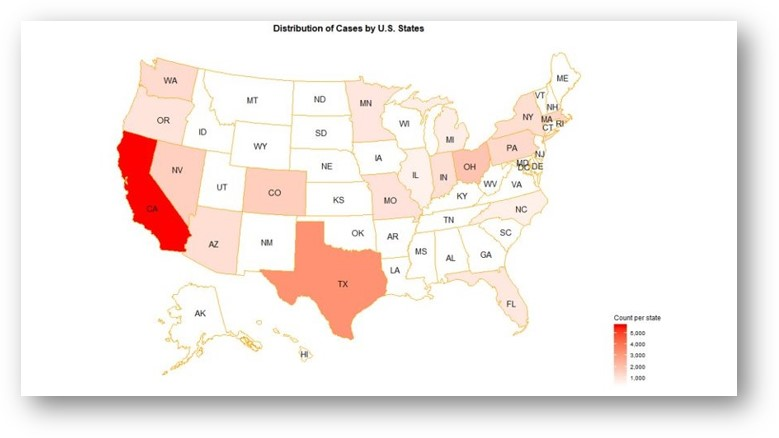
\includegraphics[width=3.5in]{Images/Figure1}
            \vspace{-15pt}
            \caption{Distribution of Cases by US states}
        \end{figure}
        \vspace{-20pt}
        \begin{figure}[H]
            \centering
            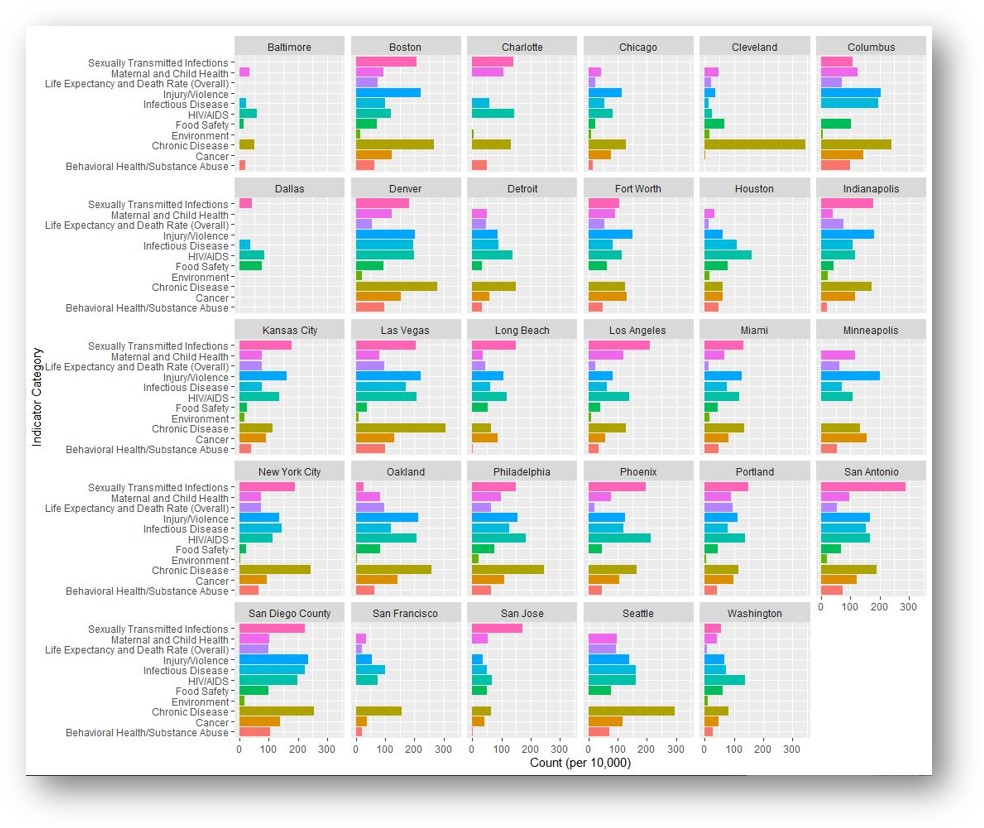
\includegraphics[width=3.5in]{Images/Figure3}
            \vspace{-15pt}
            \caption{Distribution of Cases by US Cities/Indicator}
        \end{figure}
        \begin{itemize}
            \item[-] From Figure 1 and Figure 2, we could infer that California, Texas, and Ohio are the states with highest recorded cases for all the indicator categories. Diving in the cities we found that, Los Angeles has most of the cases reported for sexually transmitted diseases, Houston for AIDS diseases, and Cleveland for Chronic Diseases.
        \end{itemize}
        \item Can we observe a trend for Indicator Categories over the years? 
        \begin{figure}[H]
            \centering
            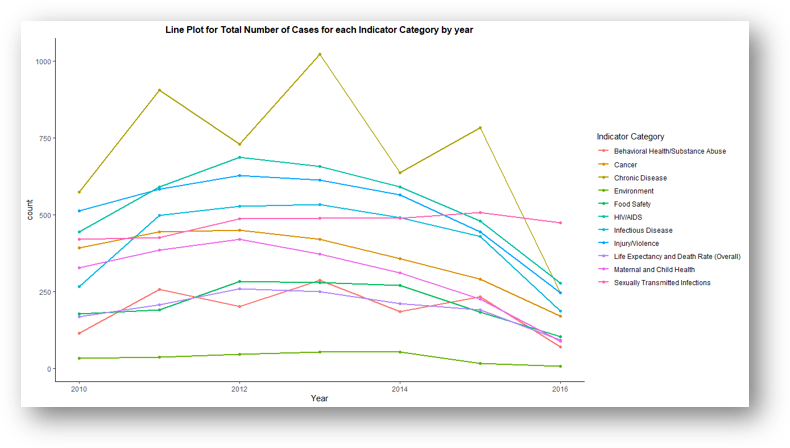
\includegraphics[width=3.5in]{Images/Figure4}
            \vspace{-15pt}
            \caption{Total Cases for Indicator/Year}
        \end{figure}
        \begin{figure}[H]
            \centering
            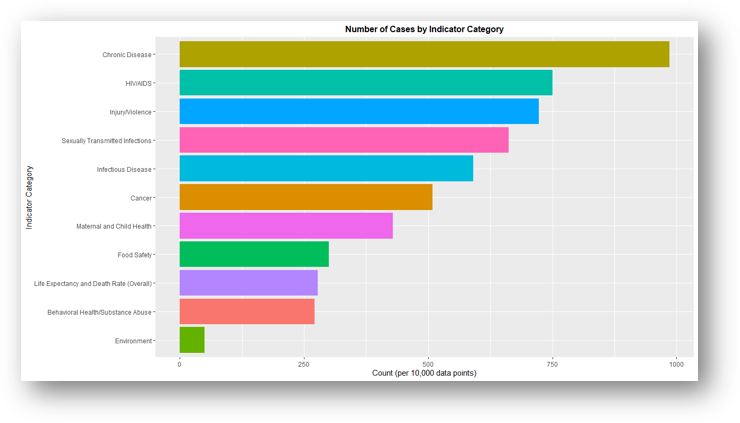
\includegraphics[width=3.5in]{Images/Figure6}
            \vspace{-15pt}
            \caption{Number of Cases/Indicator}
        \end{figure}
        \begin{itemize}
            \item[-] From the above Figures 3 and 4, we see a slight decrease in records of most categories over the years except sexually transmitted infections which show a slight increase in the recorded cases, and that Chronic diseases is the highest recorded indicator category among all. Hence, Chronic disease Indicator category becomes the category for us to dive deeper into to explore the most prevalent indicator of it.
        \end{itemize}
        \item What is the distribution of Indicators under the prevalent Indicator category (Chronic Diseases), and which Indicator is prevalent among them? 
        \begin{figure}[H]
            \centering
            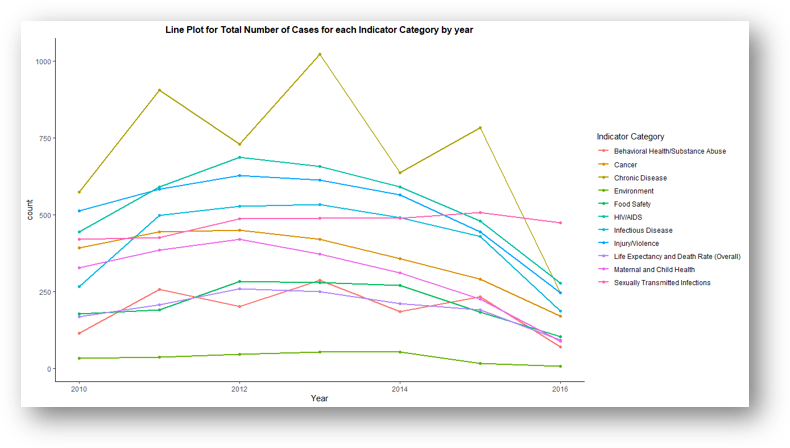
\includegraphics[width=3.5in]{Images/Figure4}
            \vspace{-15pt}
            \caption{Total Cases for Indicator/Year}
        \end{figure}
        \vspace{-15pt}
        \begin{figure}[H]
            \centering
            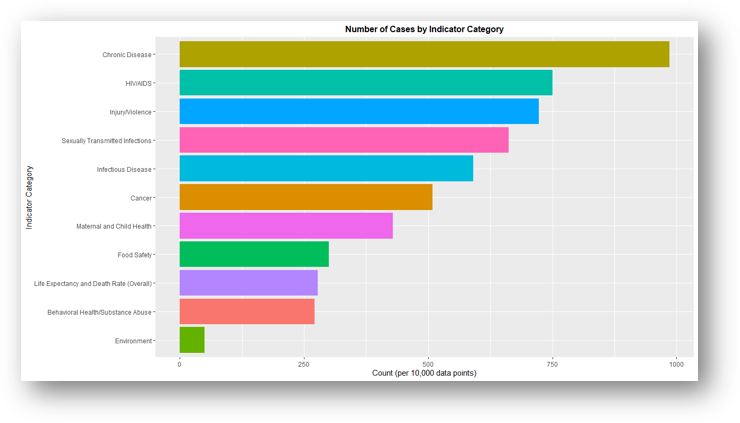
\includegraphics[width=3.5in]{Images/Figure6}
            \vspace{-15pt}
            \caption{Number of Cases/Indicator}
        \end{figure}
        \begin{itemize}
            \item[-] From Figure 5, we see that Heart disease mortality rate tops among all the indicators for Chronic Diseases, then from the Figure 6, we see that there is a significant decline in the recorded cases in the trend of all the chronic disease indicators over the years, which is unusual, and maybe a result of the data being skewed towards previous years as compared to recent years. This may have happened because of lower recent recordings of the cases by the BCHC. 
            \item[-] Thus, we used additional data set for heart disease to do CDA and PDA on Heart Disease Mortality rate (Prevalent Chronic Disease Indicator). 
        \end{itemize}
    \end{enumerate}
    \subsection{Feature Selection:}
    \subsubsection{Correlation Matrix }
    \begin{figure}[H]
        \centering
        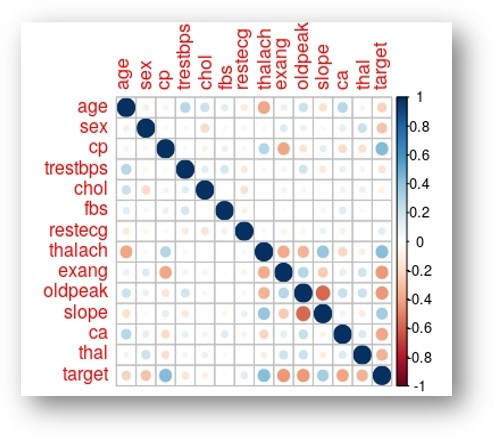
\includegraphics[width=3.5in]{Images/Figure11}
        \vspace{-15pt}
        \caption{Correlation Matrix}
    \end{figure}
    According to the Figure 7 the best predictor variable that can be seen are \textbf{cp, thalch, exang, oldpeak}. With \textbf{"cp"} and \textbf{"thalach"} giving positive correlations, while \textbf{"exang"} and \textbf{"oldpeak"} giving negative correlations. For creating the correlation matrix in R \textbf{corrplot}package was used. 
    
    \subsubsection{K-fold cross validation }
    5 fold cross validation was performed with the mean train \textbf{rmse} $0.3708088$ and mean test \textbf{rmse} of $0.3825556$.
    \vspace{-15pt}
    \begin{figure}[H]
        \centering
        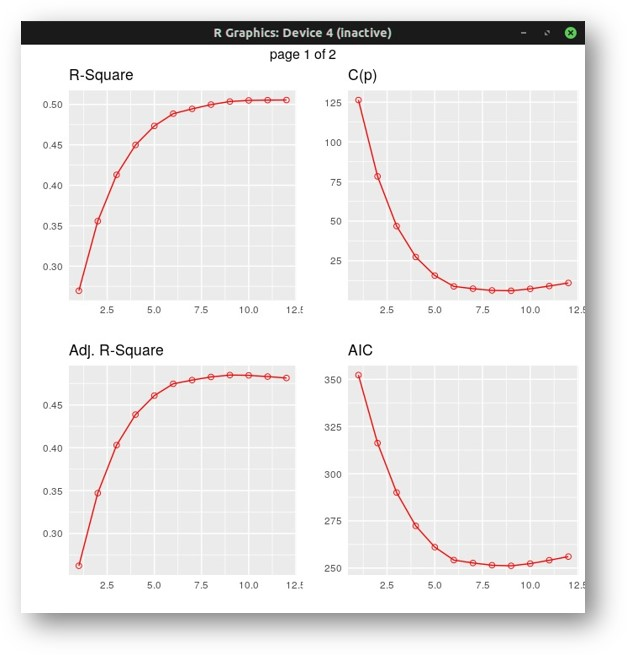
\includegraphics[width=3.5in]{Images/Figure10}
        \vspace{-15pt}
        \caption{Stepwise model section}
    \end{figure} 

    \subsubsection{Stepwise model selection}
    From Figure 8, it can be seen from the graphs that 3-4 variables are good for our model as they have low risk of over-fitting and less possibility of error. This stepwise model selection was automated by ols \cite{ols} package in R which automates the process of selection of predictor variables and runs various permutation and combinations to select the best possible order of variables and generates detailed graphs in various formats showing different kinds of errors. 

    \subsubsection{Stepwise model selection}
    \begin{figure}[H]
        \centering
        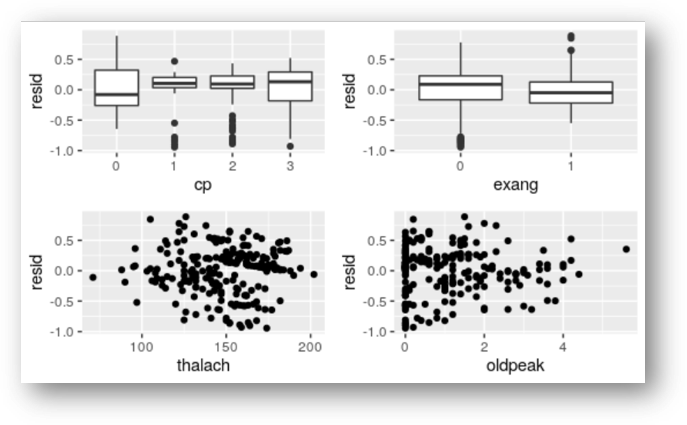
\includegraphics[width=3.5in]{Images/Figure12}
        \vspace{-15pt}
        \caption{Residuals from linear model}
    \end{figure} 
    Residuals were also generated for the selected variables over a fit on linear model to further verify the selection of right predictor variables as seen from Figure 9. \newline \newline 

    \subsection{Modelling}
    \subsubsection{Linear Model}
    \begin{figure}[H]
        \centering
        \vspace{-15pt}
        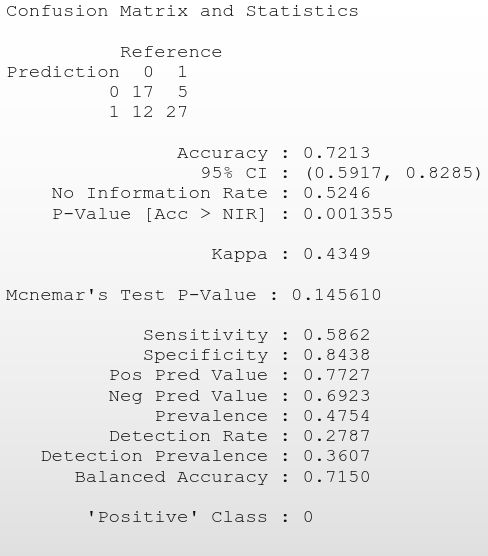
\includegraphics[width=3in]{Images/Figure13}
        \vspace{-10pt}
        \caption{Confusion Matrix: Linear Model}
    \end{figure} 
    As seen from Figure 10, with linear regression the best model achieved the accuracy of $72.13\%$. The positive likelihood ratio for this model was $3.7528$.
    \subsubsection{LSSVM}
    \begin{figure}[H]
        \centering
        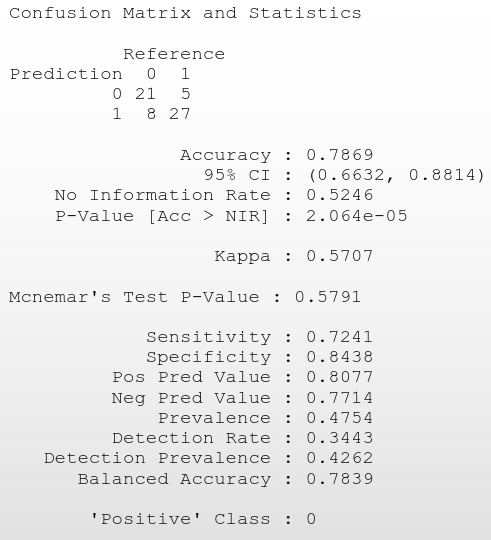
\includegraphics[width=3in]{Images/Figure14}
        \vspace{-10pt}
        \caption{Confusion Matrix: LSSVM}
    \end{figure} 
    From Figure 11 we can see that LS-SVM achieved an accuracy of $78.69\%$. Also, the positive likelihood ratio for this model is $4.63572$, which is better compared to Linear Model. 
    \subsubsection{Random Forest }
    \begin{figure}[H]
        \centering
        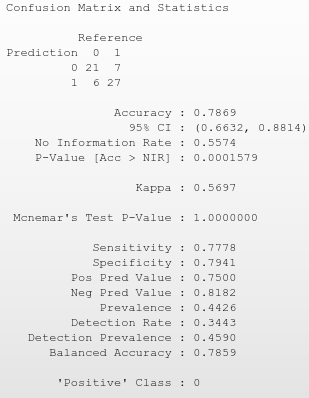
\includegraphics[width=2.9in]{Images/Figure15}
        \vspace{-10pt}
        \caption{Confusion Matrix: Random Forest}
    \end{figure} 
    As we can see in Figure 12, with Random Forest the accuracy obtained is $78.69\%$. Surprisingly it has very similar positive likelihood ratio $(Sensitivity/1-Specificity)$ for this model is $4.63572.$ 
    \subsubsection{XGBoost}
    \begin{figure}[H]
        \centering
        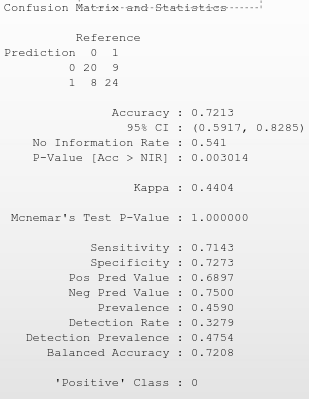
\includegraphics[width=3in]{Images/Figure16}
        \vspace{-10pt}
        \caption{Confusion Matrix: XGBoost}
    \end{figure} 
    It can be noted from Figure 13 that for XGBoost accuracy obtained XGBoost is $72.13\%$. The positive likelihood ratio $(Sensitivity/1 - Specificity)$ for this model is $2.6193$, which lowest of all.

    \section{Discussion}
    The models are compared based on 3 parameters: Accuracy, P-value and the positive likelihood ratio $(Sensitivity/1 - Specificity)$. Some models have very good accuracy however have a bad positive likelihood ratio, and hence cannot be considered as good model. The predictions from \textbf{LS-SVM} is more likely to detect the heart disease given the parameters than any other model.
    \begin{figure}[H]
        \centering
        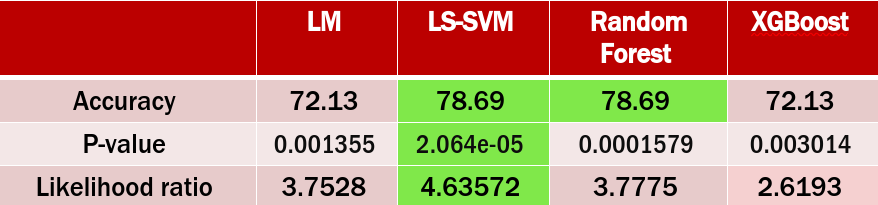
\includegraphics[width=3.6in]{Images/Figure17}
        \vspace{-5pt}
        \caption{Comparison of various Models}
    \end{figure} 
    We can conclude that, heart disease is one of the most prevalent diseases and after doing modelling on specifically heart related dataset, it is found that the most contributing factors for heart diseases is chest pressure, maximum heart graph, exercise induced angina and ST depression. It is also noted that medical data modelling can contain high error rates and model accuracies are usually on the lower side. 
    
    \section{Statement of contributions}
    It was a joint contribution by all the team members. Everyone was involved in idea development, EDA, education around models, and general discussion of approach. 
    \begin{itemize}
        \item \textbf{Prakhar Patidar} did Data Pre-processing and Exploratory Data Analysis.
        \item \textbf{Rishabh Shanbhag} worked on Data wrangling and Data visualizations.
        \item \textbf{Nikson Panigrahi} and \textbf{Kunjan Khatri} carried out Dimensionality Reduction, Computation of Correlation statistics along with implementation of Linear model, LS-SVM, Random forest and XGBoost.
    \end{itemize}   Equal contribution and efforts by all team members in preparing the presentation and final report. 

    \begin{thebibliography}{9}
        \bibitem[1]{bchc} \emph{Big Cities Health Coalition (BCHC)} 2010-2016,
        \url{https://www.bigcitieshealth.org/}. 
        \bibitem[2]{hduci} \emph{“Heart Disease UCI” Kaggle},
        \url{https://www.kaggle.com/ronitf/heart-disease-uci}
        \bibitem[3]{mlxgb} \emph{“Machine Learning with XGBoost” Kaggle},
        \url{https://www.kaggle.com/rtatman/machine-learning-with-xgboost-in-r}
        \bibitem[4]{rfr} \emph{"Random Forest in R” Towards Data Science, }
        \url{ https://towardsdatascience.com/random-forest-in-r-f66adf80ec9 }
        \bibitem[5]{ols} \emph{“Tools for Building OLS Regression Models” Cran.r project,}
        \url{https://cran.r-project.org/web/packages/corrplot/vignettes/corrplot-intro.html}
        \bibitem[6]{spgg} \emph{“Spatial Visualization with ggplot2” Cran.r project,}
        \url{https://cran.r-project.org/web/packages/ggmap/index.html}
    \end{thebibliography}
\end{multicols}
    
    \newpage
    \section*{Appendix}
    \textbf{\faicon{github} Github:} \url{https://github.com/niksnikson/idmp-bchi}

    \begin{figure}[H]
        \centering
        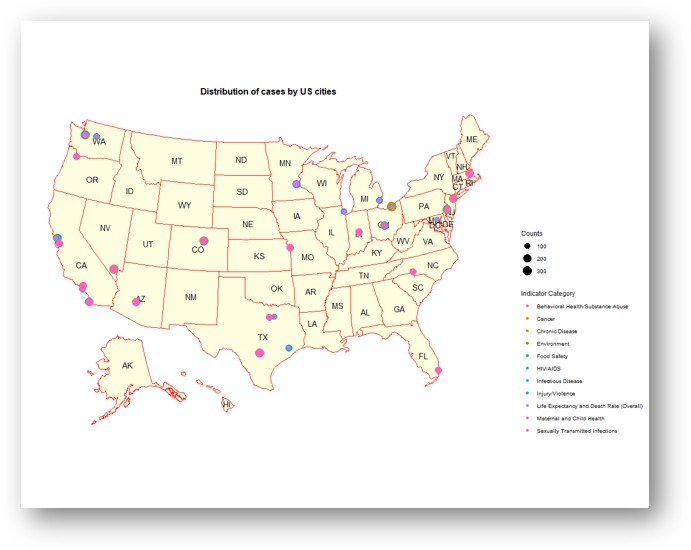
\includegraphics[width=5in]{Images/Figure2}
        \vspace{-10pt}
        \caption{Citywise Distribution}
    \end{figure} 

    \begin{figure}[H]
        \centering
        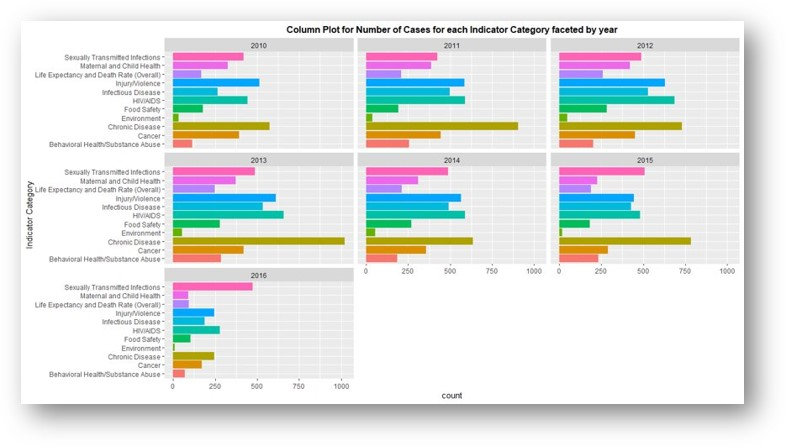
\includegraphics[width=5in]{Images/Figure5}
        \vspace{-10pt}
        \caption{Number of cases for each indicator}
    \end{figure} 
\end{document}